\chapter{FUNDAMENTOS}
\label{chap:Mt}
%\section{FUNDAMENTO TEÓRICO} 
Se dedica este capítulo a exponer los conceptos necesarios para entender el problema de investigación que se aborda.

\section{Conceptos básicos y antecedentes}

En este aparte se presentan algunos conceptos que puedes ser básicos, pero que permiten la contextualización del problema de esta tesis, así como un resumen de las publicaciones que soportar esta investigación y su aplicación en el problema que se aborda.

Preferiblemente se tomaron las referencias de los últimos 5 años, pero no se descartan otras que son básicas en este campo de investigación.

\subsection{Conceptos básicos de Grafos}
\label{ConcepGraph}
Un grafo no es otra cosa que un conjunto de vértices (al menos uno) conectados entre ellos con aristas que pueden ser líneas o flechas. 

Los grafos pueden ser dirigidos o no dirigidos, lo que gráficamente significa que sus aristas son flechas o líneas, respectivamente; si hay de ambas, se llaman grafos mixtos, como se aprecia en la tabla \ref{dirigido}.

\begin{table}[H]
\caption{Clasificación de grafos según sus aristas}
\centering
\begin{tabular}[c]{lcc}
\multicolumn{1}{c}{\textbf{TIPO}} & \textbf{DIBUJO}                      & \textbf{CARACTERÍSTICA}  \\ \hline
\multicolumn{1}{|l|}{Dirigido}    & \multicolumn{1}{l|}{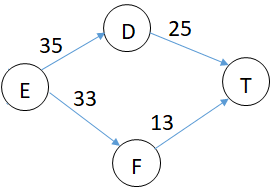
\includegraphics[align=t, width=36mm]{gafo dirigido.png} } &
%\multicolumn{1}{|l|}{Dirigido}    & \multicolumn{1}{l|}{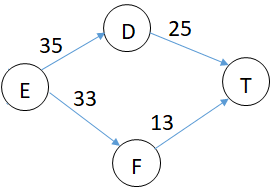
\includegraphics[width=27mm]{gafo dirigido.png} } &
\multicolumn{1}{p{6cm}|}{Todas sus aristas están dirigidas (flechas), que se pueden representar por parejas ordenadas (x,y)}     \\ \hline
\multicolumn{1}{|l|}{No dirigido} & \multicolumn{1}{l|}{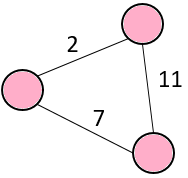
\includegraphics[align=t,width=36mm]{gafo no dirigido.png}} & \multicolumn{1}{p{6cm}|}{Todas sus aristas son no dirigidas (líneas), que se pueden representar por parejas no ordenadas \{x,y\}} \\ \hline
\multicolumn{1}{|l|}{Mixto}       & \multicolumn{1}{l|}{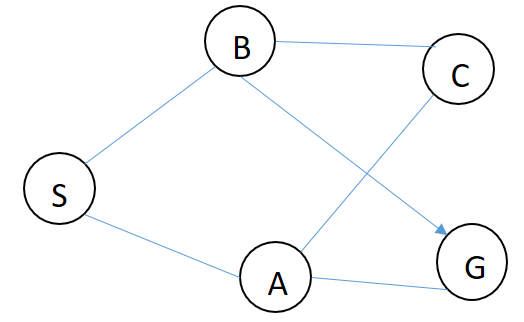
\includegraphics[align=t,width=36mm]{elementos de un grafo.png}} & \multicolumn{1}{p{6cm}|}{Contiene aristas dirigidas y aristas no dirigidas} \\ \hline
\end{tabular}
\label{dirigido}
\end{table}

Además, matemáticamente se hace una distinción en la representación de sus aristas, usándose parejas ordenas $(x,y) \in NxN$ para las aristas dirigidas y ${x,y} | (x,y) \in NxN$ para las aristas no dirigidas, lo que se puede interpretar como una doble flecha $(x,y)$ y $(y,x)$ \citep{tremblay1996matematica}.

También se habla de grafos conexos cuando no se puede separar en componentes o partes entre las que no aparecen aristas que las conecten, es decir que cada par de nodos debe estar conectado mediante un secuencia de aristas o mediante un camino.

Los grafos bipartitos son aquellos en los que se pueden diferenciar claramente dos grupos de nodos; en cada grupo de nodos no se encuentran aristas que los conecte, sino que estas van un nodo de un grupo al otro. Estos y otros conceptos sobre grafos se pueden ampliar en \citep{brandstadt1999graph}.

Estas características se cumplen en el grafo que se propone en esta tesis, además de una característica propia que se ha denominado <<grafo por etapas>>, la cual consiste en que el grafo cuenta con sus nodos distribuidos en $L$ etapas claramente diferenciadas, de forma similar a los grafos bipartitos, pero con más de dos grupos de nodos.

Esta estructura por etapas facilita el recorrido estocástico desde la primera hasta la última etapa, en orden y con probabilidades asociadas a las conexiones entre nodos, que se prestan para realizar búsquedas en el grafo, basadas en muestreo.

\subsection{Aprendizaje automático}
El Aprendizaje de Automático es una de las áreas de la Inteligencia Artificial que ha permitido extraer una importante cantidad de información, a partir de los datos que cada día se manejan en los negocios y en el mundo en general. Algunos trabajos, en este sentido, se han apoyado en diferentes técnicas como las redes Neuronales, los Algoritmos Genéticos, las Colonias de Hormigas, el Soporte de Máquina Vectorial y el Aprendizaje por Refuerzo, entre otras. 


El Aprendizaje automático se encuentra catalogado en los textos como: aprendizaje supervisado, no supervisado o mixto, aunque el aprendizaje por refuerzo - AR no se encuentra realmente en ninguna de estos tipos \citep{russell2004inteligencia}. En la tabla \ref{tipoML} se resume esta clasificación.

\begin{table}[H]
\caption{Tipos de aprendizaje automático}
\centering
\begin{tabular}{lc}
\multicolumn{1}{c}{\textbf{APRENDIZAJE}} & \textbf{CARACTERÍSTICA}                         \\ \hline
\multicolumn{1}{|l|}{Supervisado}        & \multicolumn{1}{c|}{Con datos de entrenamiento} \\ \hline
\multicolumn{1}{|l|}{No supervisado}     & \multicolumn{1}{c|}{Sin datos de entrenamiento} \\ \hline
\multicolumn{1}{|l|}{Por refuerzo}       & \multicolumn{1}{c|}{Premio o castigo}           \\ \hline
\end{tabular}
\label{tipoML}
\end{table}


En el aprendizaje supervisado el modelo aprende de acuerdo a unos datos de entrenamiento y posteriormente es capaz de reconocer patrones similares, mientras que, el aprendizaje no supervisado, no cuenta con datos de entrenamiento, sino que descubre automáticamente las características de los datos, logrando establecer, por ejemplo, las clases en las que pueden agruparse.

El AR se emplea en situaciones donde hay que tomar decisiones bajo incertidumbre, donde solo se conoce la consecuencia de una decisión después de haberla tomado. Aquí se trata de entrenar un agente inteligente, el cual debe escoger la política que mejor resultado le dé, de acuerdo a las recompensas que recibirá de un ambiente donde se encuentra inmerso \citep{sutton1992reinforcement}.

\subsection{Los Bandits}
\label{Los Bandits}

El Multiarmed-Bandit o \textit{n-armed bandits} es un modelo inspirado en las máquinas de un casino que se conocen con este nombre, donde se tienen cierto número de brazos, de los que se espera jugar los que mejor resultado alcancen. Cada máquina tiene su propia distribución de probabilidad; el jugador no las conoce inicialmente, pero a medida que va jugando, se va dando cuenta del resultado y va aprendiendo.

El modelo básico es el \textit{armed-bandit}, también conocido como \textit{bandit}, concepto que se utiliza en esta tesis, cuya analogía corresponde a una máquina de casino con un solo brazo o palanca, que en adelante se llamará acción. Para este modelo se tienen fórmulas sencillas que facilitan su implementación. 

Por ejemplo, el valor que tendrá seleccionar una acción $a$ en el tiempo $t$ se estima mediante un promedio sencillo de las recompensas que el autómata ha recibido del ambiente cada vez que seleccionó dicha acción $a$, recompensa que no necesariamente será la misma en cualquier otra oportunidad o tiempo. La fórmula que se emplea es la \ref{Q}, donde $R_i$ son los valores de recompensa que va recibiendo el autómata en cada una de las $Nt(a)$ ocasiones en que la acción $a$ fue seleccionada.
\begin{eqnarray}\label{Q}
Q_t(a) = \frac{R_1+R_2+ ...+R_{Nt(a)}}{N_t(a)}
\end{eqnarray}

Este valor asociado a cada acción, será actualizado durante el aprendizaje del autómata, es decir que para cada tiempo $t$ puede cambiar y, de él depende que la acción tenga mayor posibilidad de ser seleccionada por el autómata en ese momento, de acuerdo a lo que muestra la figura \ref{A} \citep{sutton1998introduction}.
\begin{eqnarray}\label{A}
A_t = \stackbin[a]{}{arg max}Q_t(a)
\end{eqnarray}

Así, no es completamente seguro que la acción con mejor valor sea escogida, porque estos algoritmos, y en general los del AR, hacen un balance entre la exploración y la explotación y el agente deberá decidir entre elegir acciones que ya sabe que dan un buen resultado o acciones que no ha probado o que en el pasado, no han sido las mejores; en el primer caso, para mejorar la recompensa que esa acción le ofrece y, en el segundo caso, para darse la oportunidad de encontrar acciones con mejor recompensa \citep{sutton1992reinforcement}. Una analogía de estos procesos es la búsqueda de un valor óptimo en una función; en el primer caso el agente se quedaría explorando un óptimo local y, en el segundo caso exploraría otros lugares de la función donde puede que aparezca el óptimo global.

\subsection{Antecedentes sobre Grafos}
Diferentes investigadores han propuesto aplicaciones de grafos en problemas particulares, así como la mejora o adaptación de algoritmos ya existentes.

Entre ellos, \citet{zhou2019toward} proponen mejoras a algoritmos de enrutamiento de ruta más corta (Shortest Path Routing - SPR), mediante sondeos de rutas múltiples y aprendizaje colaborativo. Citan, además, trabajos en esta misma área como el de \citet{liu2012adaptive} quienes aplican los principios del Bandido Multi-Brazos con brazos independientes, al problema presentado por \citet{liu2011multi}, quienes pretenden recomendar la mejor ruta en un grafo, desde un origen hasta un destino, donde el costo de cada enlace individual no se puede ver y el costo total de extremo a extremo solo se puede observar al finalizar el recorrido y está dado por la suma de los costos de todos los enlaces en la ruta. 

Un problema similar, conocido como \textit{Online Shortest Path Problem}, es abordado como trabajo de grado por \citet{AvilaCartes2018}, mediante el uso de un grafo dirigido y sin ciclos, con un nodo inicial y uno final o nodo sumidero. La solución aprovecha los alcances del \textit{n-armed.bandit}, pero, además de minimizar el costo con el camino que se seleccione, busca disminuir la cantidad de veces que se escoge uno que presente fallas.

Otra tesis donde se recogen problemas de aplicación de grafos y \textit{bandits}, es la de \citet{valko2016bandits} quien se esfuerza por mostrar la aplicación de modelos que investigadores han desarrollado en problemas reales, valiéndose de los grafos y cómo hacer uso de los desarrollos en \textit{n-armed-bandit}.

Es el caso de \cite{tossou2017thompson}, ellos proponen un algoritmo para problemas de decisión secuenciales, con grafos que presentan altos grados de incertidumbre, basado en los enunciados de \citet{thompson1933likelihood}, como alternativa para las decisiones que se toman basados en sencillos cálculos de probabilidades, donde uno de dos eventos queda aceptado y el otro descartado. 

Se cita también una propuesta de investigadores en inteligencia artificial de IBM \citep{lakshmanan2010predictive} que modelan un caso semiestructurado de Gestión de Procesos de Negocios, mediante un grafo cuyos nodos son las actividades y sus aristas indica si hay flujo entre cada par de nodos. Se tiene la información de quienes son los vecinos de cada nodo y una probabilidad de pasar a cada uno de ellos, las cuales deben sumar 1; estas son las probabilidades que la aplicación va a ir modificando hasta encontrar una sola secuencia de actividades para dar solución al caso; dicha modificación sigue las reglas de las feromonas de los algoritmos de Optimización con Colonia de Hormigas para encontrar cuál nodo ha de recibir la recompensa y para actualizar todas las probabilidades de acceder a los vecinos de un nodo. A medida que van disminuyendo los valores de las probabilidades para algunas aristas, también llegará el momento en que algunos nodos ya no sean tenidos en cuenta.

En este trabajo como en otros, el grafo propuesto no implica mayores características que ser un grafo conexo y dirigido, con un nodo origen y un nodo final establecidos, sin encontrar en dichos trabajos las características del grafo por etapas, objeto de esta tesis. 

Un resumen de esta revisión bibliográfica se presenta en la tabla \ref{tab:litera1}
\begin{table}[h] 
\caption{Revisión de literatura - Grafos}
\centering
\begin{tabular}{cc}
\textbf{FUENTE}   & \textbf{DESCRIPCIÓN}   \\ \hline
\multicolumn{1}{|l|}{\citet{zhou2019toward}} & \multicolumn{1}{p{10cm}|}{Proponen mejoras a algoritmos de enrutamiento de ruta más corta (SPR), mediante sondeos de rutas múltiples y aprendizaje colaborativo.} \\ \hline
\multicolumn{1}{|l|}{\citet{liu2011multi}}   & \multicolumn{1}{p{10cm}|}{Recomendar la mejor ruta en un grafo, desde un origen hasta un destino donde el costo de cada enlace individual no se puede ver y el costo total de extremo a extremo solo se puede observar al finalizar el recorrido y está dado por la suma de los costos de todos los enlaces en la ruta. No hay etapas con nodos disyuntos.} \\ \hline
\multicolumn{1}{|l|}{\citet{liu2012adaptive}}   & \multicolumn{1}{p{10cm}|}{Aplican los principios del Bandido Multi-Brazos con brazos independientes al problema presentado por \citet{liu2011multi}} \\ \hline
\multicolumn{1}{|l|}{\citet{AvilaCartes2018}}   & \multicolumn{1}{p{10cm}|}{Problema \textit{Online Shortest Path Problem}, donde se usa un grafo dirigido y sin ciclos, con un nodo inicial y uno final o nodo sumidero. Haciendo uso de \textit{n-armed.bandit}, además de minimizar el costo con el camino que se seleccione, se desea disminuir la cantidad de veces que se escoge uno que presente fallas.} \\ \hline
\multicolumn{1}{|l|}{\citet{valko2016bandits}}   & \multicolumn{1}{p{10cm}|}{Recoge problemas de aplicación de grafos y \textit{bandits}, mostrando la aplicación de modelos que investigadores han desarrollado en problemas reales} \\ \hline
\multicolumn{1}{|l|}{\citet{tossou2017thompson}}   & \multicolumn{1}{p{10cm}|}{Algoritmo para problemas de decisión secuenciales, con grafos que presentan altos grados de incertidumbre, como alternativa para cuando las decisiones se tomaban basados en sencillos cálculos de probabilidades, quedando uno de dos eventos aceptado y el otro descartado.} \\ \hline
\end{tabular}
\label{tab:litera1}
\end{table}

%Se exploró entonces la aplicación que se ha hecho de \textit{bandits} en problemas modelados por grafos, encontrando que muchos de ellos han aportado a los actuales modelos de toma de decisiones llamados sistemas de recomendación.
\subsection{Antecedentes sobre aprendizaje por refuerzo}
Muchas investigaciones se han dado para mejorar o adaptar los métodos de aprendizaje por refuerzo a diferentes situaciones.

Una propuesta para mejorar el tiempo de decisión de un algoritmo \textit{AQ-learnig} de aprendizaje por refuerzo con técnicas de inteligencia artificial de búsqueda por colonia de hormigas, se puede consultar en \citep{lee2005reinforcement}.

Se encuentra también la propuesta de \citet{alon2017nonstochastic}, quienes, mediante los principios de Regresión, crean un espectro de modelos cuya complejidad está entre la de los problemas donde el agente conoce únicamente la recompensa de las acciones luego de que las va eligiendo, y la de los problemas donde el agente tiene la información de lo que ocurrirá con cualquier acción candidata en cualquier instante de tiempo.

De otra parte, \citet{alon2015online} modelan el problema de un jugador aleatorio que se encuentra dentro de un ambiente adversario, de forma que después de cada acción, el jugador recibe de sus vecinos información binaria del efecto de su acción, que le permitirá mejorar sus próximas decisiones.

\citet{gokcesu2018online} presentan un algoritmo para \textit{n-armed bandits} con complejidad lineal que crece en función de la cantidad de secuencias posibles y del número de rondas del juego, sin el conocimiento del brazo que se debería escoger y sin suposiciones estadísticas.

Así mismo, en \citep{8170860} se encuentra un modelado de un problema de aprendizaje por refuerzo, mediante grafos, no con el esquema tradicional de la secuencia de los brazos seleccionado, sino que es un grafo en el que los nodos sí representan los brazos, pero las aristas tiene que ver con la similitud de sus valores de recompensas, lo que es aplicable a los sistemas de recomendación. El modelo les permitió presentar un algoritmo con baja complejidad. 

Como \citet{alon2017nonstochastic} y \citet{xu2017online}, muchos autores han hecho propuestas para mejorar el desempeño de algoritmos existentes, en cuanto a su complejidad o al campo de solución que influyen, utilizando técnicas de aprendizaje por refuerzo en el escenario de los \textit{bandits}. En general, se trabaja con un \textit{m-armed bandit}, donde los nodos representan los brazos y, las aristas, dirigidas o no dirigidas, relacionan los nodos.

Y, finalmente, no se puede dejar de mencionar el trabajo de \citet{silver2017mastering} y los predecesores de \textit{AlphaZero} \citep{silver2016mastering} que revolucionaron al mundo con la aplicación de técnicas de aprendizaje por refuerzo para mejorar el entrenamiento conseguido con redes neuronales de aprendizaje profundo, que logró derrotar a los mejores jugadores humanos de ajedrez y Go, entre otros juegos, cada vez con mejores resultados.

De esta forma se puede apreciar que en la revisión hecha, no se encuentra una propuesta que combine los aspectos del aprendizaje por refuerzo de los \textit{m-armed bandit}, con un grafo que tenga como restricción que la acción seguida a ejecutar deba pertenecer a la etapa siguiente de la anterior, como lo contempla la propuesta de esta tesis.
%\section{Gestión de Procesos de Negocio}

Un resumen de esta revisión bibliográfica se presenta en la tabla \ref{tab:litera2}

\begin{table}[!h] 
\caption{Revisión de literatura - Aprendizaje por refuerzo}
\centering
\begin{tabular}{cc}
\textbf{FUENTE}   & \textbf{DESCRIPCIÓN}   \\ \hline
\multicolumn{1}{|l|}{\citet{lee2005reinforcement}} & \multicolumn{1}{p{10cm}|}{Propuesta para mejorar el tiempo de decisión de un algoritmo \textit{AQ-learnig} de aprendizaje por refuerzo con técnicas de inteligencia artificial de búsqueda por colonia de hormigas.} \\ \hline
\multicolumn{1}{|l|}{\citet{alon2017nonstochastic}}   & \multicolumn{1}{p{10cm}|}{Mediante los principios de Regresión, crean un espectro de modelos cuya complejidad está entre la de los problemas donde el agente conoce únicamente la recompensa de las acciones luego de elegirlas, y la de aquellos donde el agente tiene la información de lo que ocurrirá con cualquier acción candidata en cualquier instante.} \\ \hline
\multicolumn{1}{|l|}{\citet{alon2015online}}   & \multicolumn{1}{p{10cm}|}{Modelan el problema de un jugador aleatorio que se encuentra dentro de un ambiente que puede ser su adversario, quien después de cada acción recibe de sus vecinos información binaria del efecto de su acción.} \\ \hline
\multicolumn{1}{|l|}{\citet{gokcesu2018online}}   & \multicolumn{1}{p{10cm}|}{Presentan un algoritmo para \textit{n-armed bandits} con complejidad lineal que crece en función de la cantidad de secuencias posibles y del número de rondas del juego, sin el conocimiento del brazo que se debería escoger y sin suposiciones estadísticas.} \\ \hline
\multicolumn{1}{|l|}{\citet{8170860}}   & \multicolumn{1}{p{10cm}|}{Modelado de un problema de aprendizaje por refuerzo, mediante grafos, con un grafo en el que los nodos sí representan los brazos, pero las aristas tiene que ver con la similitud de sus valores de recompensas, aplicable a los sistemas de recomendación con baja complejidad} \\ \hline
\multicolumn{1}{|p{4cm}|}{\citet{silver2017mastering} y \citet{silver2016mastering}}   & \multicolumn{1}{p{10cm}|}{Aplicación de técnicas de aprendizaje por refuerzo y redes neuronales de aprendizaje profundo, que lograron derrotar a los mejores jugadores humanos de ajedrez y Go, entre otros juegos, cada vez, con mejores resultados.} \\ \hline
\end{tabular}
\label{tab:litera2}
\end{table}

Luego de estas revisiones se procede a describir las bases matemáticas que soportan el modelo \textit{L-n-armed-bandits}, para que se constituya en una propuesta novedosa que se sume a las muchas que se han generado para contribuir cada día a una mejor toma de decisiones, para las personas y para las aplicaciones mismas.

\section{Denominación del modelo propuesto}
\label{nombre}

\textit{El algoritmo propuesto se ha llamado \textit{L-n-armed bandit} ya que se basa en el algoritmo \textit{n-armed bandit} para un grafo por etapas (ya definido), cuya cantidad está representada por la letra $L$}

\textit{Cabe resaltar que este grafo ha de contener la cantidad de etapas $L$ que el problema a modelar requiera, así como los nodos de cada etapa y las conexiones entre nodos de etapas seguidas; sin embargo, para el desarrollo de la propuesta se generarán de forma aleatoria algunos de estos valores, cuya digitalización puede resultaría tediosa en cada una de las pruebas a que se someta.}

\textit{Esta estructura por etapas facilita el recorrido estocástico desde la primera hasta la última etapa, en orden y con probabilidades asociadas a las conexiones entre nodos, lo que se presta para realizar búsquedas en el grafo, basadas en muestreo. Para conseguir estas probabilidades se aprovecha la forma de operar del algoritmo \textit{n-armed bandit}.}

\textit{Cada uno de los nodos del grafo será en realidad un \textit{bandit} con un valor o utilidad desconocido que solo se podrá ir estimando al terminar la selección de los L nodos de todas las etapas del grafo, ya que en la última etapa es donde se recibe algún refuerzo positivo o negativo, de acuerdo al conjunto de nodos seleccionados de cada etapa.}

\textit{Las forma como se generan valores y se simulan los refuerzos, así como las bases matemática que soportan la propuesta se describen en seguida.}

\section{Fundamentos matemáticos}

Como ya se ha mencionado, se pretende usar un modelo estructurado que aproxime los valores de una matriz de probabilidades de transición de estados, que se relacionen con los valores de utilidad que en un momento dado tengan los nodos candidatos a ser visitados.

Un modelo de probabilidades de transición de estados se adapta al problemas de búsqueda en el grafo por etapas con cualquier cantidad de nodos y remplazaría la forma de seleccionar una acción que se explicó para los \textit{bandits} en las ecuaciones \ref{Q} y \ref{A} \citep{sutton1998introduction}.

También se ha de tener en cuenta que, la probabilidad total de una secuencia determinada de nodos, equivale a multiplicar las probabilidades de ir de un nodo a otro hasta culminar la ruta, tal como se hace en un árbol Bayesiano y como se presenta en la fórmula \ref{modelp1}.
\begin{eqnarray}
\label{modelp1}
P(i_{0} \to i_{1}, ... i_{l-1} \to i_{l}, ... i_{L-1} \to i_{L})=P(i_{0} \to i_{1})P(i_{1} \to i_{2})...P(i_{L-1} \to i_{L}),
\end{eqnarray}
donde $i$ denota el nodo seleccionado en cada una de las etapas, su subíndice $l=0,1,...,L$ denota la etapa a la que pertenece y L denota el número total de etapas. 

La fórmula \ref{for:2}, como sucede con la distribución de \textit{Boltzman}, permite normalizar las probabilidades para que correspondan a cantidades positivas menores o iguales a 1, pero con un fácil cálculo de la sudatoria del denominador, dados los valores de A que corresponden a ceros o a unos. 

\begin{eqnarray}\label{for:2}
P(i \to j) = \frac{e^{v_j}}{\sum_k A_{i,k} e^{v_k}},
\end{eqnarray}


Así, la cantidad del numerador siempre será inferior o,  a lo sumo, igual a la cantidad del denominador, dado que el numerado es parte de la sumatoria del denominador, que, adicionalmente, es de valores positivos. La multiplicación por el valor de cada posición en la matriz de adyacencia $A$, garantiza que únicamente se sumen los exponenciales de nodos a los que en realidad se accede. 

Otra característica de esta fórmula es que con los valores iniciales en cero para los exponentes de $e$, se obtienen probabilidades uniformes para todo nodo $j$ adyacente al nodo $i$.

Finalmente, para controlar el aprendizaje del autómata se incrementa o decrementa el valor del exponente de la fórmula anterior, dado que de esta forma aumenta o disminuye la probabilidad asociada al nodo relacionado. Esto puede verse en la fórmula sencilla \ref{for:3}.
\begin{eqnarray}\label{for:3}
v_j(\tau + 1) = v_j(\tau) + \delta,
\end{eqnarray}

donde $\delta$ es un parámetro que controla la rata de aprendizaje:

$P(i \to j)_{\tau+1} \sim e^{\delta} P(i \to j)_{\tau}$ 

para pequeños valores de $\delta$.

\section{Proceso de negocio}

Aunque la definición de proceso es algo que está en la mente de cualquiera de los lectores, se define aquí un proceso de negocio como un conjunto de actividades ejecutadas en una secuencia específica, es decir, que tiene un flujo determinado por la lógica del negocio, los eventos externos y las reglas del negocio \citep{hitpass2017bpm}, para dar un contexto inicial del contenido de este capítulo. A partir de este concepto se derivan los que aquí se exponen.

\subsection{Gestión de procesos de negocio}

BPM es el acrónimo de Business Process Management, en español: Gestión de Procesos de Negocio. Es una disciplina que integra un conjunto de principios, métodos y tecnologías con el propósito de contribuir al mejoramiento continuo del funcionamiento empresarial.

La idea de BPM es hacer visible la gestión de los procesos de negocio y facilitar los cambios que sean requeridos \citep{smith2003business}.

Según \citet{garimella2008introduccion}, BPM hace referencia a un conjunto de mejores prácticas de gestión de procesos, herramientas y tecnologías utilizadas para diseñar, representar, analizar y controlar los procesos del negocio, combinando las tecnologías de la información con metodologías de proceso y gobierno.

BPM incluye el soporte integral de las tecnologías de información para mejorar, innovar y gestionar los procesos que determinan los resultados del negocio, crean valor para el cliente y facilitan el logro ágil de los objetivos del negocio” \citep{abpmp2013v3}.

\subsubsection{Suite de gestión de procesos de negocio bpms}

Un sistema o suite para la gestión de procesos de negocios (Business Process Management Suite (BPMS) “es un conjunto de herramientas de software que permiten modelar implementar y gestionar los procesos de negocio, que abarcan múltiples aplicaciones empresariales, departamentos y \textit{partners}”\citep{smith2003business}.

Una Suite de Gestión de Procesos de Negocio está conformada por herramientas de software para la gestión de los procesos de negocios (diseño de procesos, flujo de trabajo, aplicaciones, integración y supervisión), los cuales son automatizados favoreciendo a las organizaciones \citep{underdahl2013gestion}.

\subsection{Proceso de negocio dinámico y caso}

Es un proceso de negocio que no tiene un orden determinado para la ejecución de las actividades, ni la certeza de cuáles de ellas se han de ejecutar, requiriendo la intervención de un experto \citep{hitpass2017bpmn}. 

El término \textit{case}, que en \cite{van2005case} se define como una situación que puede ocurrir en una organización, para la cual el procedimiento de resolución no está necesariamente predefinido.

A la tecnología que se encarga de la gestión de este tipo de procesos se le conoce momo gestión de “casos”; el caso contiene toda la información sobre el proceso \citep{marin2016introduction}.

%\section{Modelo y notación de procesos de negocio}

%Las notaciones BPMN y CMMN que se describen en este apartado, son grafos de actividades y otros elementos que indican la secuencia de tareas que se siguen para que la BPMS guíe el desarrollo de un proceso, este hecho es el que motiva que se puede orientar el modelo al grafo que aquí se expone, aplicando una estrategia particular que permita trasladar toda la información necesaria.

%\subsection{BPMN}

%Business Process Model and Notation (BPMN) es una herramienta gráfica estandarizada, para la notación del modelado de procesos de negocio, mediante un flujo de trabajo.

%La versión BPMN 2.0 fue presentada en el año 2011 \citep{omg2011business} y utiliza símbolos, relaciones y atributos para el modelado de procesos de negocio. Un ejemplo gráfico de cómo se ve un proceso modelado en BPMN se muestra en la figura \ref{EjBPMN}.

%Una recopilación de conceptos de modelado de procesos y los elementos que componen cada modelo, son ampliados por \citet{lemusenfoque}.

%\begin{figure}[H]
  %\centering
   % 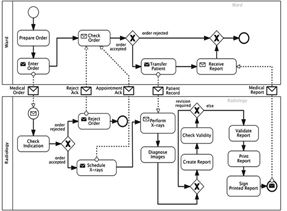
\includegraphics[scale=1.5]{EjBPMN.png}
  %\caption[Modelado de un proceso estructurado]{Modelado de un proceso estructurado con BPMN}
  %\label{EjBPMN}
%\end{figure}

\subsection{CMMN}
\label{Sec:CMMN}

Uno de los estándares emergentes para el modelado de casos es Case Management Model and Notation (CMMN), que utiliza un conjunto de símbolos gráficos, reglas de composición y artefactos para este propósito; una descripción completa de esta notación se encuentra en \cite {Cmmn}, pero se enfatiza que las líneas de puntos alrededor de las actividades las hacen opcionales y esto revela la incertidumbre que caracteriza a los casos.

Case Management Model and Notation” – CMMN es una referenciación entregada por el grupo “Object Management Group” (OMG), como una notación gráfica para la gestión de casos y procesos dinámicos \citep{hauder2014research}; algunas de sus principales diferencias con la notación de procesos de negocio deterministas se ilustra en \citet{breitenmoser2015case}. \citet{auer2014business} también fundamenta y explica la notación CMMN.

\begin{figure}[h]
  \centering
    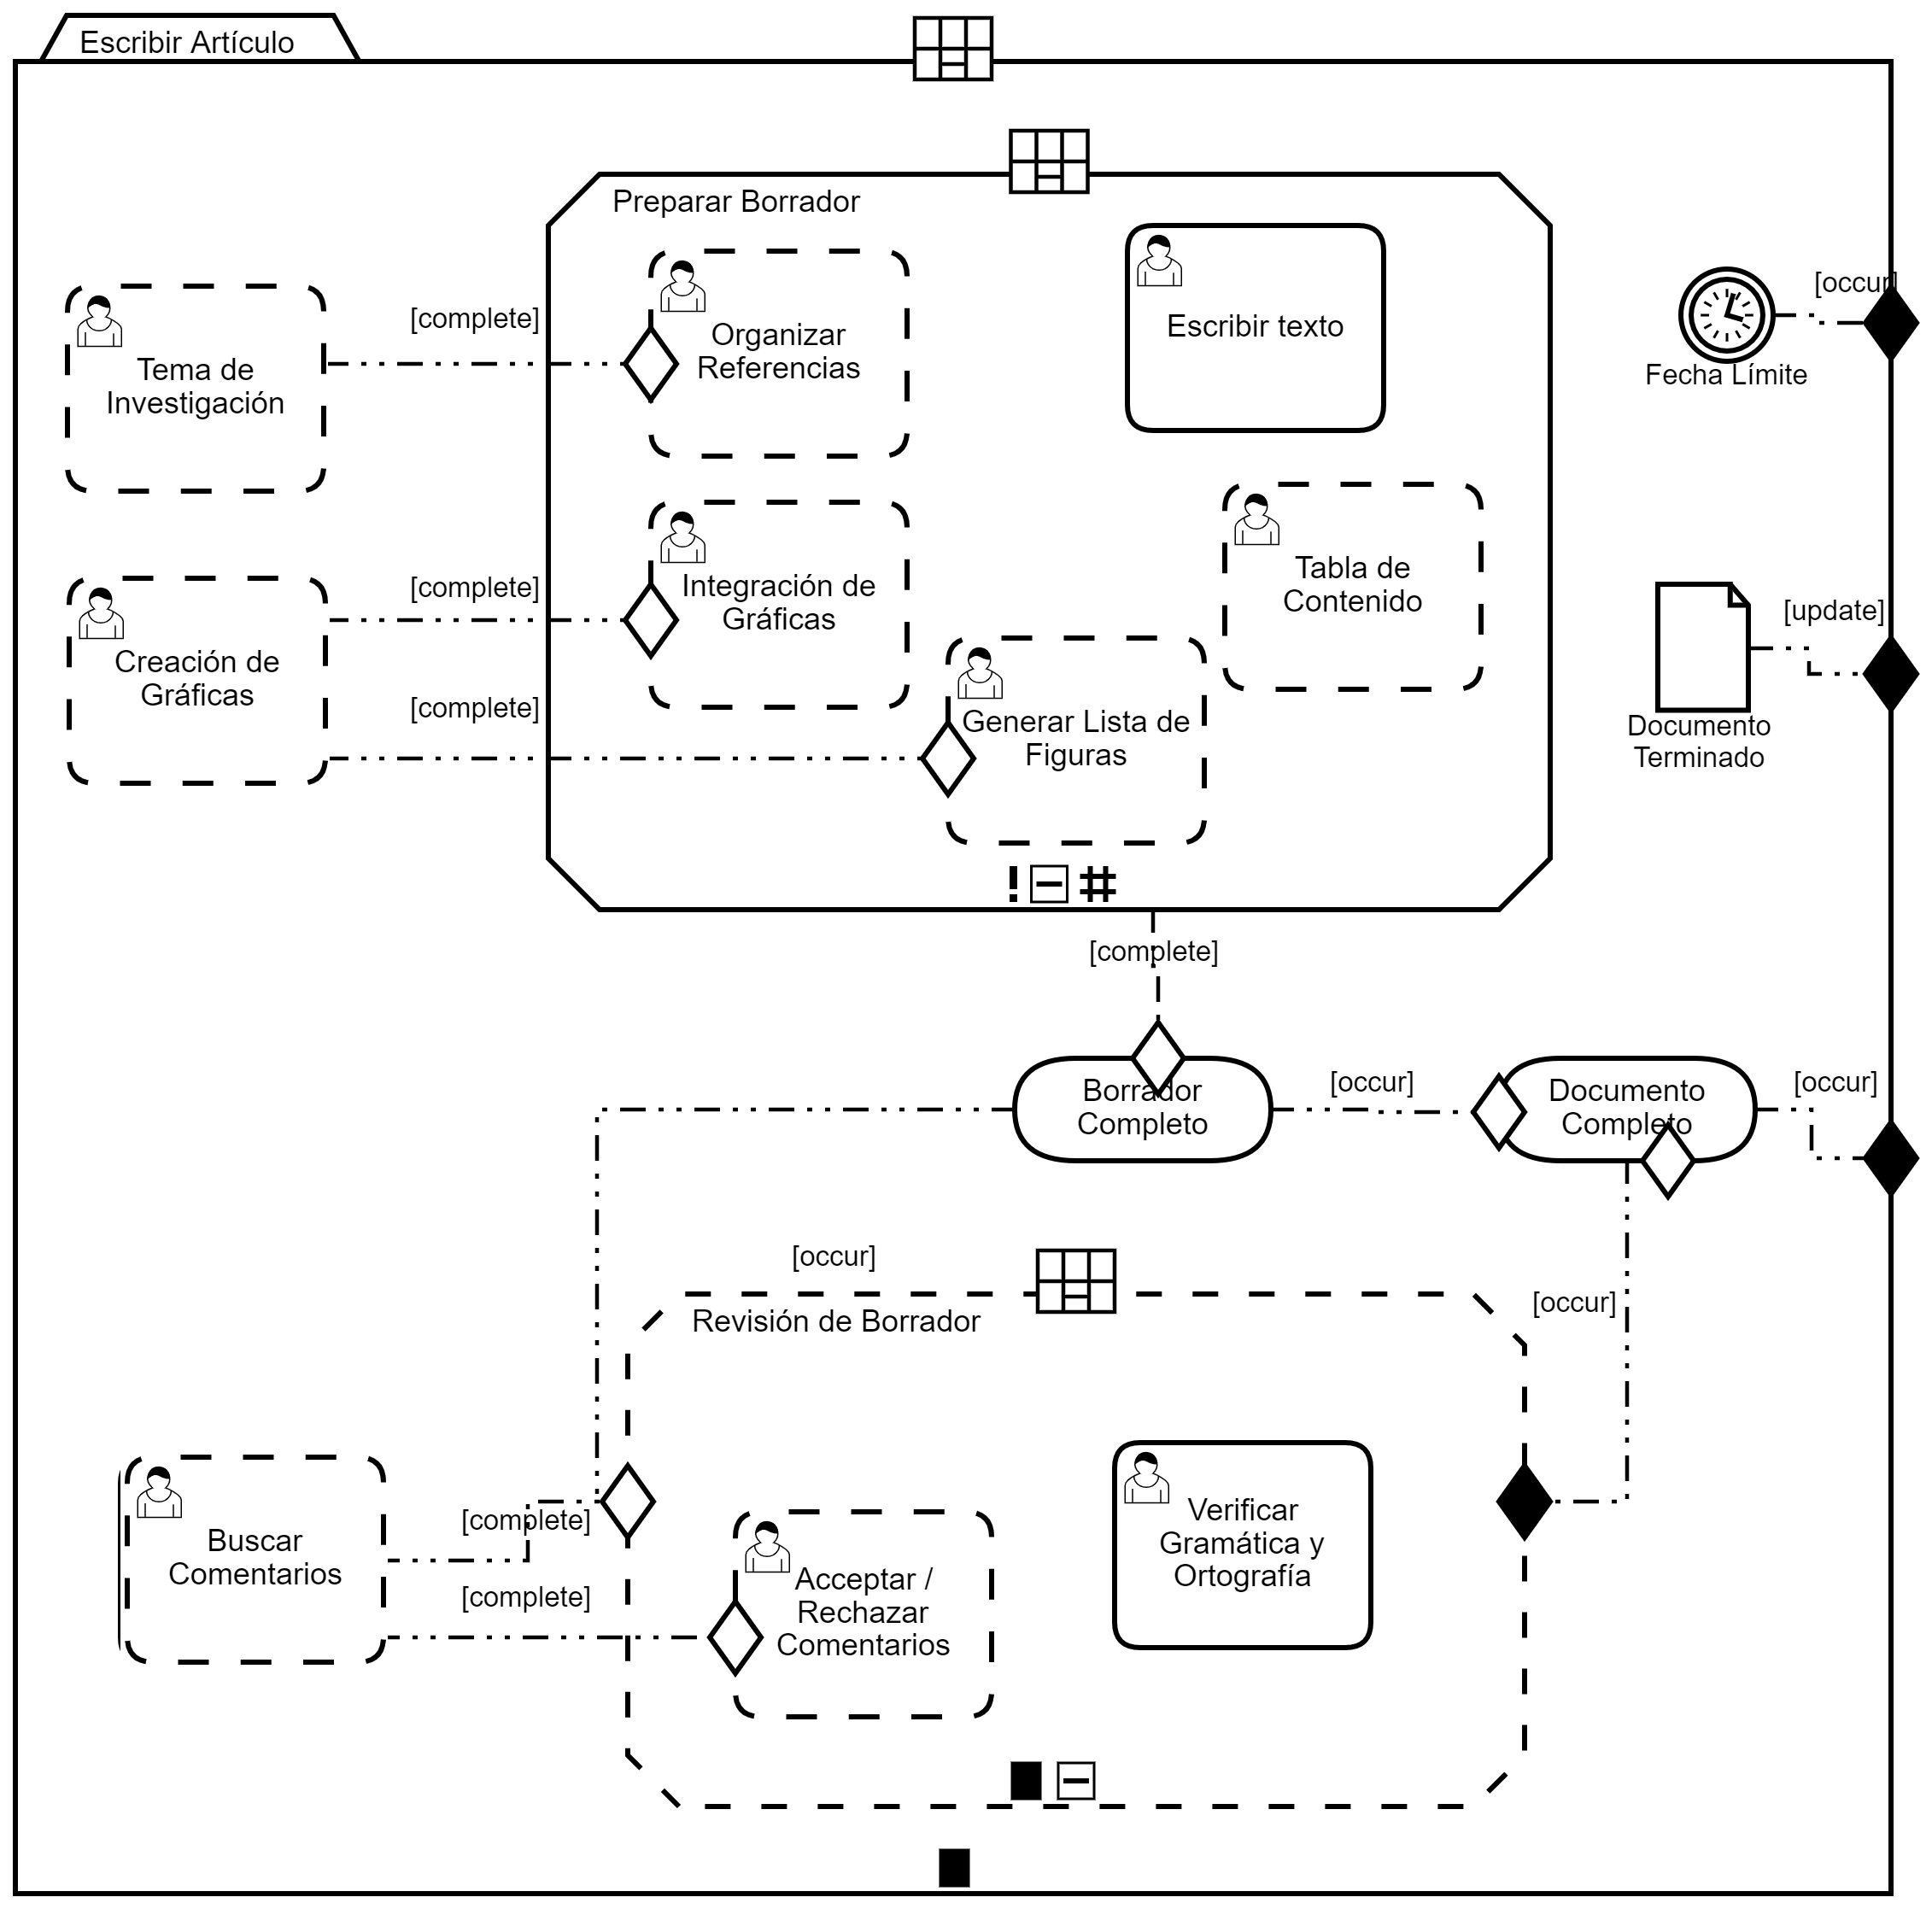
\includegraphics[scale=0.25]{ModeloCMM.png}
  \caption[Modelado de un proceso dinámico]{Modelado de un proceso dinámico con CMMN}
  \label{EjCMMN}
\end{figure}

En \citet{marin2016introduction} se da una aplicación de esta notación a un sistemas de atención de quejas. \citet{breitenmoser2015case} presenta un modelo en notación CMMN para seleccionar candidatos que aplica a un proceso de naturalización en un gobierno local. Tanto en \citet{auer2014business}  como en \citet{omg2011business} se expone una adaptación del ejemplo que se ve n la figura \ref{EjCMMN}, el cual corresponde al proceso de escribir un documento.

%\subsection{Modelo CMMN en un grafo por etapas}

Al hacer la comparación de la notación para el modelado de los procesos estructurados contra la notación de los procesos dinámicos, en el ejemplo que se adaptó de \citet{Cmmn11}, se establece que las líneas punteadas de la figura \ref{EjCMMN} representan la incertidumbre en cuanto a la secuencia que se puede seguir, e incluso a la presencia o no de algunas actividades en la solución a la que se llegue.

%Se vislumbra entonces, cómo esta notación CMMN puede llevarse a un grafo con etapas (como el de la figura \ref{GrafoEtapas}) donde se pueda modelar la incertidumbre en la selección de tareas, disponiendo para cada etapa un conjunto de actividades, de las que no se conoce su probabilidad de ser seleccionada, quedándole al algoritmo de aprendizaje por refuerzo que se implementa para el grafo, el trabajo de recomendar la tarea a seguir después de haber ejecutado alguna tarea de la etapa anterior, restringiendo la selección de una única tarea en cada etapa.

%Para esto se propone que, si dos actividades o tareas b y c están después de una actividad a, pero b y c no son disjuntas, entonces se deben ofrecer b y c en cualquiera de las etapas siguientes, ya que fusionarlas en un nodo ficticio no permite esclarecer con certeza sus prerrequisitos. 

%En este ejercicio, es necesario traer de alguna forma la información pasada, por si alguna actividad que es predecesora de otras se ha ejecutado en etapas anteriores, pero no necesariamente en la inmediatamente anterior. Para ellos es preciso activar una bandera cuando se ejecute una actividad que sea predecesora de otras y condicionar al programa a que revise la bandera, cuando vaya a seleccionar una de las actividades posteriores.

%Un caso específico se presenta en el apéndice \ref{apendicecaso}, el cual se constituye como una parte del trabajo de investigación en el manejo de casos dinámicos de las BPMS que concibió el ingeniero Luis Chaparro, al interior del grupo de investigación GIPROCAS de la Universidad de Boyacá en Colombia.

%Dada esta introducción al caso de estudio, se procede a presentar las consultas bibliográficas correspondientes para establecer si el grafo propuesto ya se encuentra en otra investigación y si ya ha sido abordado un modelo cercano al \textit{L-n-armed-bandits}.
